\chapter{Workload Characterization}
Il dataset di partenza è composto da \textbf{3000 righe} e \textbf{24 colonne}, ciascuna delle quali rappresenta uno dei parametri del sistema oggetto di studio. Si tratta di parametri caratterizzanti l'esecuzione di vari Threads su un sistema operativo.
\\In particolar modo le colonne con prefisso $Vm$ rappresentano informazioni sulla memoria virtuale occupata e utilizzata dai Threads, mentre le altre colonne rappresentano informazioni di carattere generale, come memoria libera, numero di threads, pagine inattive ecc.

\section{Filtraggio}

\subsection{Colonne Identiche}
Innanzitutto osservando il workload e effettuando un grafico delle distribuzioni è possibile rendersi conto della presenza di ben 4 colonne costanti:
\begin{itemize}
	\item \textbf{Active}
	\item \textbf{AnonPages}
	\item \textbf{AvbLatency}
	\item \textbf{Error}
\end{itemize}
Tali colonne in quanto costanti non spiegano varianza, dunque possono essere tranquillamente trascurate ai fini dell'analisi.
\\Osservando le distribuzioni dei parametri \textbf{WriteBack} e \textbf{MemFree} si sono notate alcune caratteristiche comuni. Per avere una maggiore chiarezza si è preferito calcolare la matrice delle correlazioni su questi due parametri.
\begin{figure}[H]
	\centering
	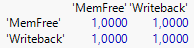
\includegraphics{img/hw1/correlazione_mem_writeback.png}
	\caption{\textit{Matrice di correlazione tra MemFree e WriteBack}}
\end{figure}
Osservando la matrice appare evidente che le due colonne sono esattamente identiche, fornendo quindi la stessa informazione. Per questo motivo si è deciso di trascurare una delle due, in particolare quella di WriteBack.
\\Le 24 colonne iniziali sono state ridotte a 19 colonne, riducendo il dataset di un numero di osservazioni pari a:
\begin{equation}
	n_{dati} = 3.000 \times (24 - 19) = 15.000
\end{equation}

\subsection{Outlier}
Gli outliers sono valori anomali all'interno dell'insieme di osservazioni, in altre parole sono valori che si discostano notevolmente dagli altri valori dell'insieme. 
Essendo valori anomali la loro frequenza di occorrenza è bassa rispetto agli altri valori e ciò li porta ad essere identificati all'esterno del range interquartile. 
In alcuni casi gli outlier possono essere eliminati ma ciò è possibile solo a monte di una analisi accurata. Tali valori infatti influiscono sulle analisi statistiche in modo considerevole e non sempre rappresentano situazioni trascurabili per l'analisi da svolgere .
Osservando attraverso box plot e grafici di distribuzione l'andamento dei seguenti parametri :
\begin{itemize}
	\item \textbf{VmSize} (quanta memoria virtuale utilizza l'intero processo);
	\item \textbf{VmHWM} (di quanta RAM il processo necessita al massimo);
	\item \textbf{VmRSS} (quanta RAM il processo sta correntemente usando);
	\item \textbf{VmPTE} (quanta memoria Kernel è occupata dalle entries della tabella delle pagine);
\end{itemize}
\begin{figure}[H]
	\centering
	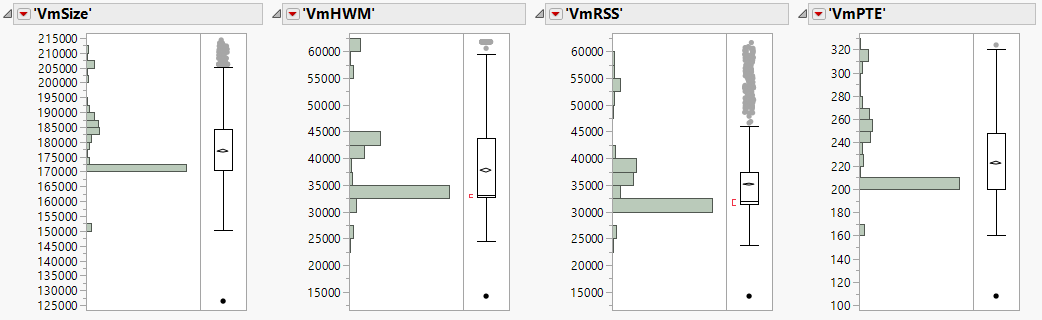
\includegraphics[width=1\textwidth]{img/hw1/outlier_vm.png}
	\caption{\textit{Grafici di distribuzione di VmSize, VmHWM, VmRSS, VmPTE}}
\end{figure}
Si è notato che essi presentano un outlier isolato (in basso ad ogni grafico) in comune associato alla prima riga del dataset. Analizzando gli altri parametri (\textit{MemFree}, \textit{Dirty}, \textit{PageTables}, \textit{Buffer}, ...) è stato possibile evidenziare che anche per la maggior parte di essi lo è, ma non è un punto isolato. 
\\L'ipotesi fatta è che con molta probabilità le prime righe del dataset (da 0 a 100 circa), rappresentano la fase di avvio del processo e l'outlier oggetto di studio è la prima istanza di questa fase. Dato che l'obiettivo della caratterizzazione del workload è quello di analizzare le prestazioni a regime del sistema oggetto di studio (in questo caso), si è deciso di trascurare quel singolo outlier. Tuttavia è bene notare che in ogni caso le informazioni riguardo questa fase di avvio non saranno del tutto perse dato che è stato rimosso un singolo punto e non tutti i punti che la rappresentano.
\\
\vspace{0.5cm}
\\
Un secondo outlier che può essere agevolmente rimosso è la riga 512 in cui il parametro \textbf{Slab} assume valore 4. 
\begin{figure}[H]
	\centering
	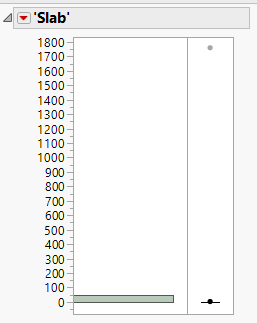
\includegraphics[width=0.4\textwidth]{img/hw1/outlier_slab1.png}
	\caption{\textit{Grafico di distribuzione di Slab}}
\end{figure}
Oltre ad avvicinarsi molto al valore medio assunto da Slab (zero), esso risulta essere un outlier solo per il parametro stesso dato che per gli altri è un valore compreso tra i quartili. Una sua rimozione quindi non influenza gli indici di caratterizzazione sintetica dei parametri del workload complessivo.
\\
\vspace{0.5cm}
\\
Un terzo outlier è il valore 1760 del parametro \textit{Slab}, associato alla riga 90 del workload.
\begin{figure}[H]
	\centering
	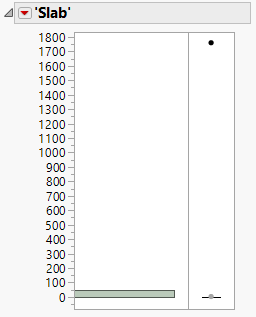
\includegraphics[width=0.4\textwidth]{img/hw1/outlier_slab2.png}
	\caption{\textit{Grafico di distribuzione di Slab}}
\end{figure}
Rispetto al precedente, tale outlier richiede un' analisi più approfondita visto che influenza significativamente l'andamento di parametri quali \textit{Mapped} e \textit{PageTables}. Per descrivere meglio la dipendenza tra questi parametri si può effettuare un grafico tra il numero dell'osservazione e il valore assunto da \textit{Mapped}, analogo discorso con \textit{PageTables}.	
\begin{figure}[H]
	\centering   
	\subfigure{	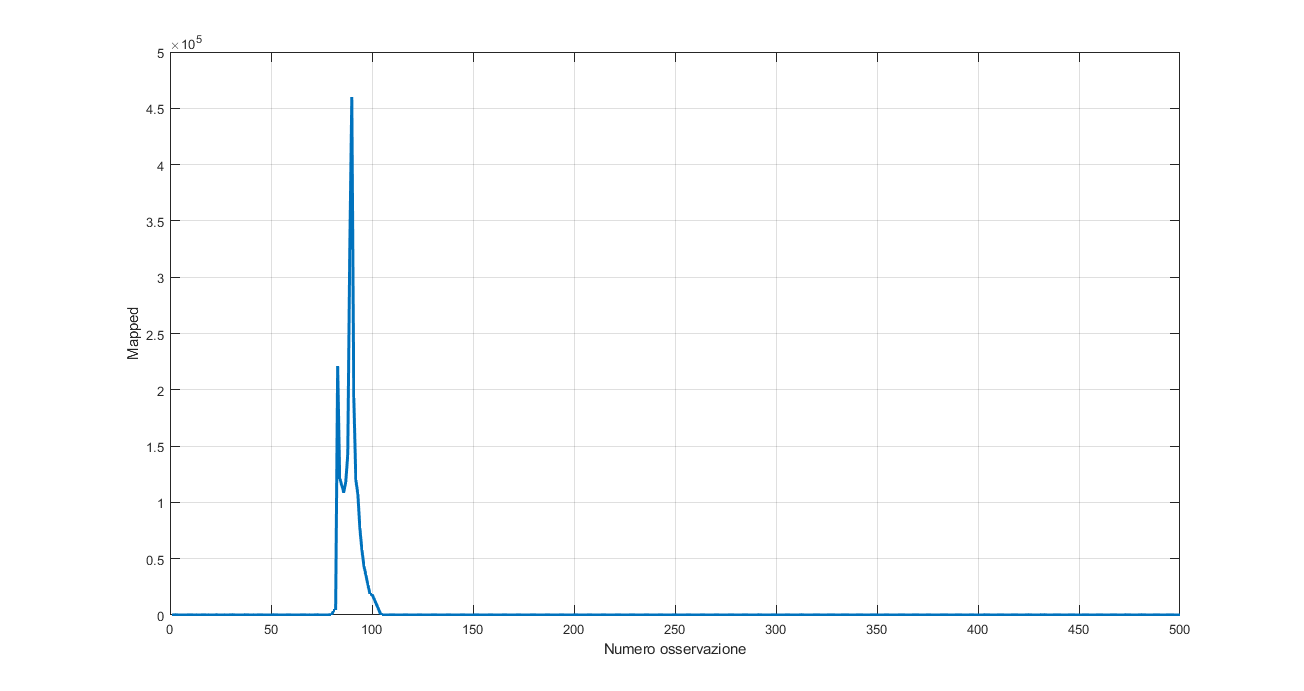
\includegraphics[width=\textwidth]{img/hw1/mapped.png}}
	\caption{\textit{Grafico tra numero di osservazione e valore assunto dal parametro Mapped}}
	\subfigure{	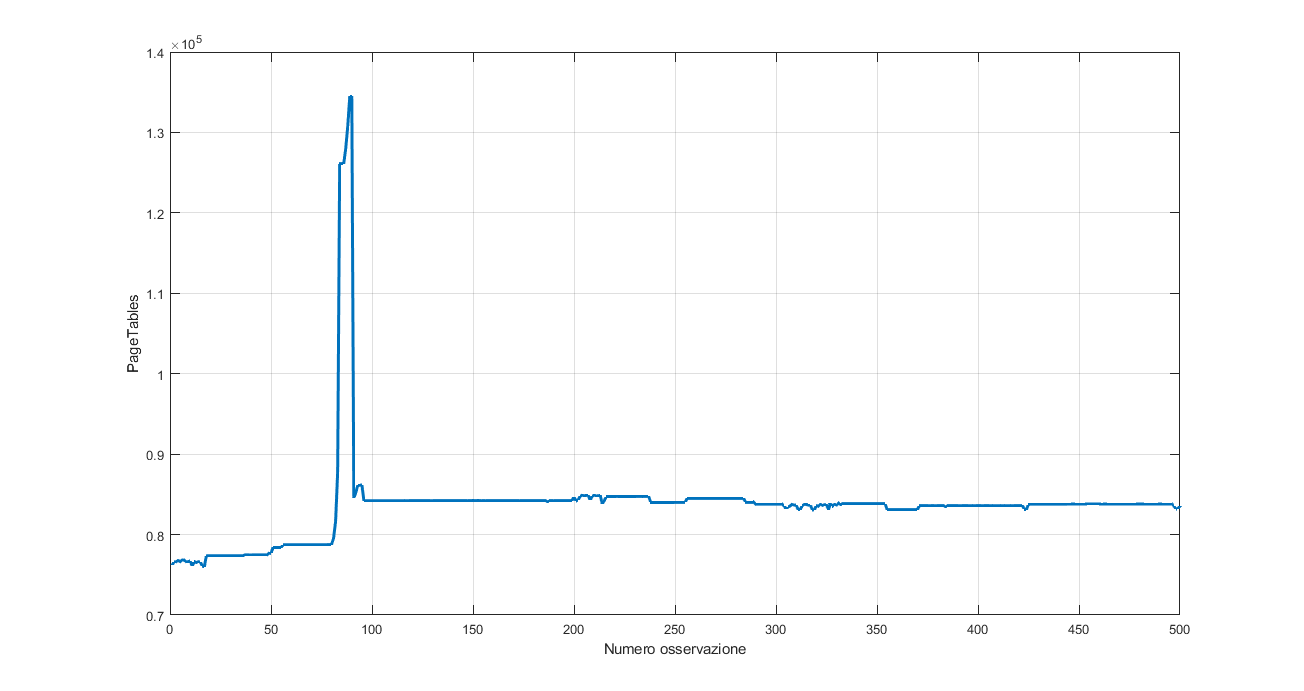
\includegraphics[width=\textwidth]{img/hw1/pagetables.png}}	
	\caption{\textit{Grafico tra numero di osservazione e valore assunto dal parametro PageTables}}
\end{figure}
Si nota che in corrispondenza (in realtà nell'osservazione appena precedente) dell'outlier del parametro \textit{Slab} i due parametri sopra indicati hanno un picco, durante la fase di avvio del sistema.
\\Lo Slab si riferisce ad un particolare meccanismo di allocazione/deallocazione della memoria nel Kernel. Dato che influenza in particolar modo altri parametri si è preferito non trascurarlo.\\
In conclusione sono stati eliminati dal dataset solo 2 outlier che corrispondono a 38 osservazioni. Quindi il dataset è stato ridotto in totale di 15.038 elementi, provocando una diminuzione dei dati iniziali di poco più del $20\%$.
\newpage

\section{PCA}
A seguito del filtraggio il dataset risulta ridotto grazie alla rimozione di alcune colonne che non esprimevano varianza e alcune righe rappresentanti outlier trascurabili.
\\Su questo dataset si possono quindi iniziare a fare le prime considerazioni.
\\Utilizzando la tecnica della \textit{Principal Component Analysis} il dataset può essere estremamente ridotto, sfruttando solo le \textit{Componenti Principali} che mantengono più varianza. Il risultato della PCA è quindi:
\begin{figure}[H]
	\centering
	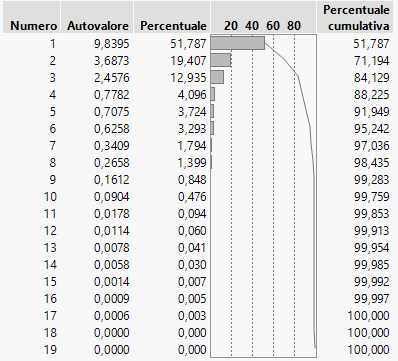
\includegraphics{img/hw1/pca.png}
	\caption{\textit{PCA applicata al dataset filtrato}}
\end{figure}
La scelta del numero di componenti principali ricade in particolar modo sulla devianza che quelle componenti mantengono rispetto al dataset reale. Inoltre essa dipende anche dal tipo di osservazioni ed esperimento che è stato effettuato.
\\In questo caso la scelta è ricaduta sul prendere 5 componenti principali poiché rappresentano il 92\% della devianza totale. Esso rappresenta un valore abbastanza elevato, ma è stato scelto per mantenersi in una regione di tolleranza durante la clusterizzazione. 
\\Anche se il workload sintentico verrà costruito considerando 5 componenti principali, in seguito sono riportati i risultati di PCA e clusterizzazione anche nel caso in cui fosse stato scelto un numero diverso di componenti principali, ovvero:
\begin{itemize}
	\item Prendere 4 PC
	\begin{equation*}
		DEV_{PCA-MANTENUTA} \approx 88 \%
	\end{equation*}
	\item Prendere 5 PC
	\begin{equation*}
			DEV_{PCA-MANTENUTA} \approx 92 \%
	\end{equation*}
	\item Prendere 6 PC
	\begin{equation*}
			DEV_{PCA-MANTENUTA} \approx 95 \%
	\end{equation*}
\end{itemize}
Per ognuno di questi 3 insiemi di Principal Components è stata effettuata la procedura di clustering .

\section{Clustering}
Il clustering è una tecnica che consiste nel raggruppare osservazioni "simili" tra loro. La similitudine tra un elemento e un cluster, o tra un cluster e un altro cluster, può essere calcolata secondo varie tecniche. In questa analisi si è preferito utilizzare il \textbf{metodo di Ward}, il quale pesa la distanza tra due cluster in relazione al numero di elementi che li compongono.
\\Dati due cluster P e Q (un elemento non appartenente ad un cluster, può essere visto come un cluster di dimensione 1), sia $|P|$ la cardinalità di $P$, analogo con $|Q|$, e sia $\bar{x}_p$ il centroide di $P$, analogo con $\bar{x}_q$, la distanza tra $P$ e $Q$ viene calcolata come:
\begin{equation*}
	d(P,Q) = 2 \dfrac{|P| \; |Q|}{|P| + |Q|} ||\bar{x}_p - \bar{x}_q ||^2
\end{equation*}
Per ogni raggruppamento viene poi scelto una singola osservazione che la rappresenta, riducendo quindi il numero di righe del dataset pari al numero di cluster scelti durante l'analisi.
\\Il numero di cluster da scegliere può dipendere da vari fattori:
\begin{itemize}
	\item Omogeneità dei cluster: i cluster devono raggruppare un numero di osservazioni quanto il più possibile omogeneo rispetto agli altri cluster. Avere un cluster con un numero di elementi di vari ordini di grandezza rispetto ad un altro cluster non sempre può portare a buoni risultati (in termini di devianza).
	\item Devianza mantenuta: a seguito della PCA parte della devianza nei dati viene persa. Dato che il clustering viene effettuato sulle \textit{Componenti Principali} allora esso produce un'ulteriore perdita di devianza nel risultato finale.
\end{itemize}
\subsubsection{Devianza Persa}
Per effettuare il calcolo della devianza totale persa persa bisogna prima calcolare la devianza intra-cluster (la somma delle devianze per ogni cluster) e sulla base di questa si può calcolare la quantità richiesta.
\\Matematicamente, definita $DEV_{PCA-PERSA}$ la devianza persa (in termini percentuali) a causa della PCA, viceversa $DEV_{PCA-MANTENUTA}$ la devianza mantenuta dalla PCA, e $DEV_{INTRA}$ la devianza intra-cluster, la devianza totale persa percentuale vale:
\begin{equation*}
	DEV_{PCA-LOST} + DEV_{INTRA}\times DEV_{PCA-MANTENUTA}
\end{equation*}
Essa può essere calcolata in MATLAB passando ad uno script i cluster, le componenti principali e il dataset iniziale.
\\ Per dare valore ai fattori sopra citati il clustering viene effettuato scegliendo un numero di cluster che varia da 6 a 16 (per ogni gruppo di componenti principali) su cui poi viene calcolata la devianza persa.
\newpage
 \subsection{4 Componenti Principali}
 Utilizzando le prime quattro PC si ha:
 \begin{figure}[H]
 	\centering   
 	\subfigure{	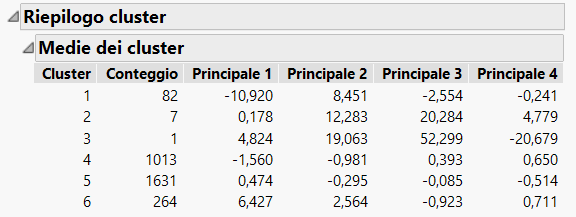
\includegraphics[width=0.30\textwidth]{Homework/Workload_Characterization/PCA_&_Clustering/4_Comp/Clustering/6_Cluster/Screen_Dati/Riepilogo.png}}
 	\subfigure{	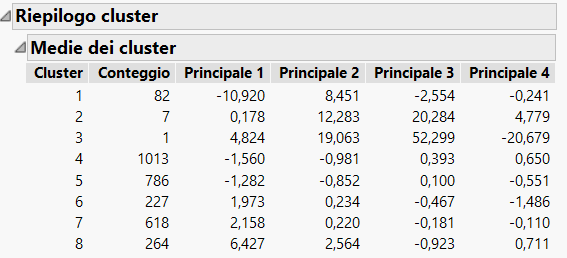
\includegraphics[width=0.30\textwidth]{Homework/Workload_Characterization/PCA_&_Clustering/4_Comp/Clustering/8_Cluster/Screen_Dati/Riepilogo.png}}
 	\subfigure{	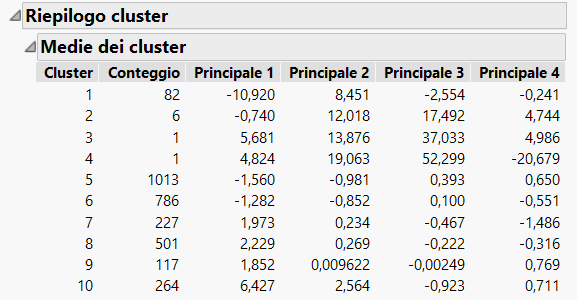
\includegraphics[width=0.30\textwidth]{Homework/Workload_Characterization/PCA_&_Clustering/4_Comp/Clustering/10_Cluster/Screen_Dati/Riepilogo.png}}
 	\subfigure{	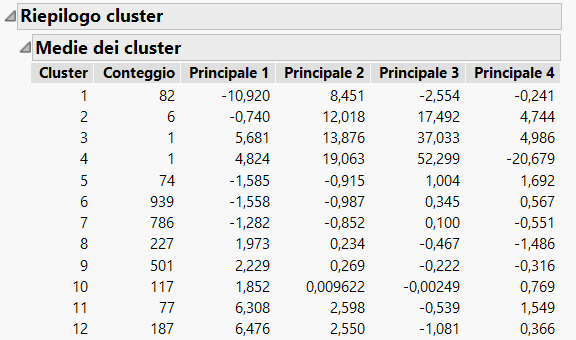
\includegraphics[width=0.30\textwidth]{Homework/Workload_Characterization/PCA_&_Clustering/4_Comp/Clustering/12_Cluster/Screen_Dati/Riepilogo.png}}
 	\subfigure{	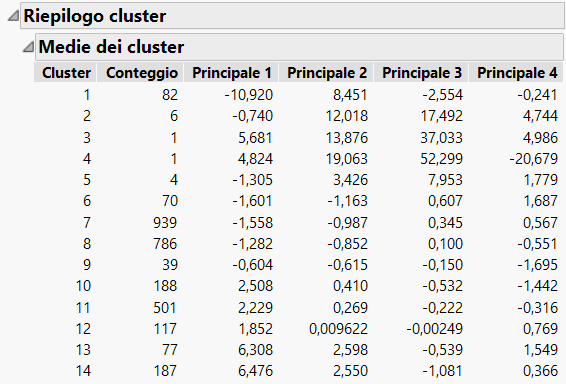
\includegraphics[width=0.30\textwidth]{Homework/Workload_Characterization/PCA_&_Clustering/4_Comp/Clustering/14_Cluster/Screen_Dati/Riepilogo.png}}
 	\subfigure{	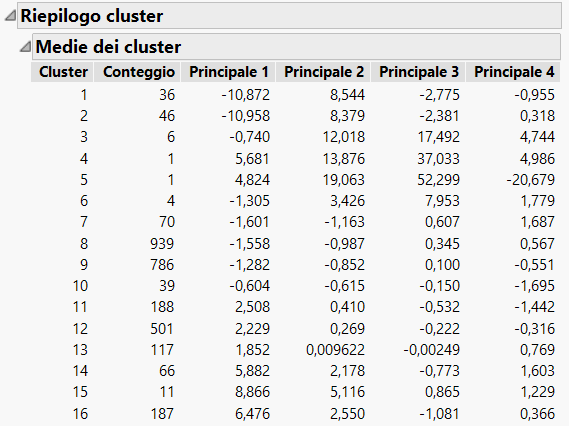
\includegraphics[width=0.30\textwidth]{Homework/Workload_Characterization/PCA_&_Clustering/4_Comp/Clustering/16_Cluster/Screen_Dati/Riepilogo.png}}
 	\caption{\textit{Numero di cluster e dimensione per diversi valori}}
 \end{figure}
La devianza persa durante la clusterizzazione varia in relazione al numero di cluster scelti. Si possono racchiudere le informazioni in un'unica tabella:
\begin{center}
	\begin{tabular}{|c|c|c|c|c|c|}
		\hline
		\textbf{6 Cluster} & \textbf{8 Cluster} & \textbf{10 Cluster} &\textbf{12 Cluster}& \textbf{14 Cluster} & \textbf{16 Cluster} \\
		\hline
		26\%& 17\% & 16\% & 15\% & 14.5\% & 14\% \\
		\hline
	\end{tabular}
\end{center}
\vspace{0.5cm}
 \subsection{5 Componenti Principali}
 Utilizzando le prime quattro PC si ha:
 \begin{figure}[H]
 	\centering   
 	\subfigure{	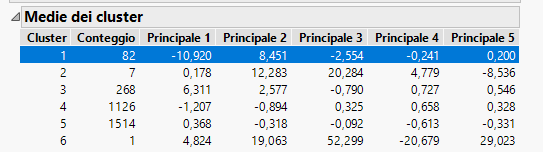
\includegraphics[width=0.30\textwidth]{Homework/Workload_Characterization/PCA_&_Clustering/5_Comp/Clustering/6_Cluster/Screen_Dati/Riepilogo.png}}
 	\subfigure{	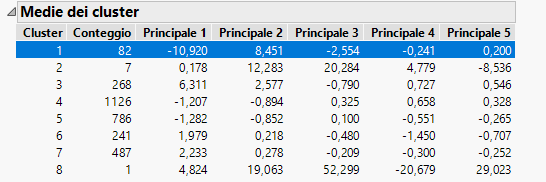
\includegraphics[width=0.30\textwidth]{Homework/Workload_Characterization/PCA_&_Clustering/5_Comp/Clustering/8_Cluster/Screen_Dati/Riepilogo.png}}
 	\subfigure{	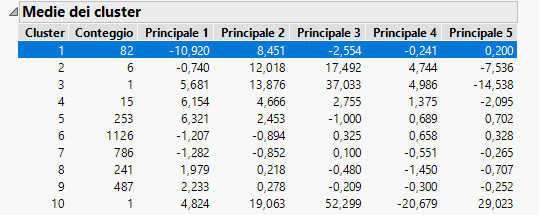
\includegraphics[width=0.30\textwidth]{Homework/Workload_Characterization/PCA_&_Clustering/5_Comp/Clustering/10_Cluster/Screen_Dati/Riepilogo.png}}
 	\subfigure{	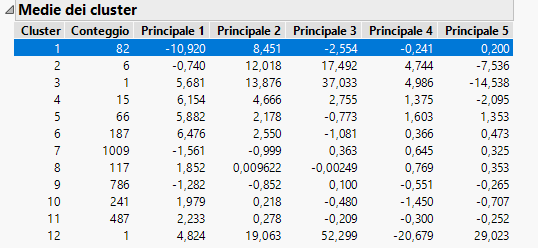
\includegraphics[width=0.30\textwidth]{Homework/Workload_Characterization/PCA_&_Clustering/5_Comp/Clustering/12_Cluster/Screen_Dati/Riepilogo.png}}
 	\subfigure{	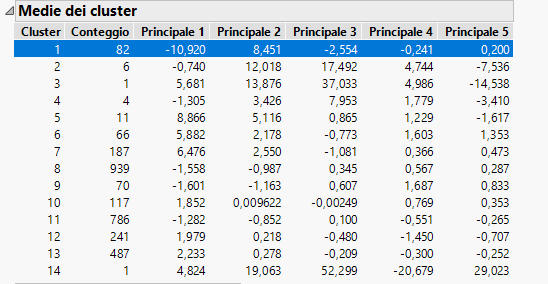
\includegraphics[width=0.30\textwidth]{Homework/Workload_Characterization/PCA_&_Clustering/5_Comp/Clustering/14_Cluster/Screen_Dati/Riepilogo.png}}
 	\subfigure{	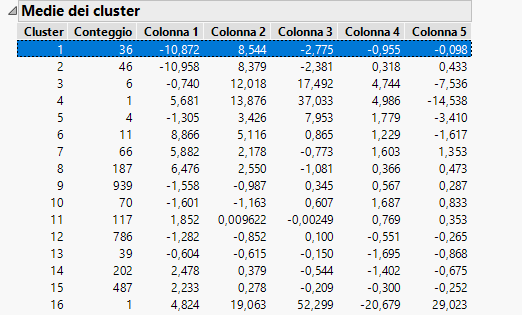
\includegraphics[width=0.30\textwidth]{Homework/Workload_Characterization/PCA_&_Clustering/5_Comp/Clustering/16_Cluster/Screen_Dati/Riepilogo.png}}
 	\caption{\textit{Numero di cluster e dimensione per diversi valori}}
 \end{figure}
La devianza persa durante la clusterizzazione varia in relazione al numero di cluster scelti. Si possono racchiudere le informazioni in un'unica tabella:
\begin{center}
	\begin{tabular}{|c|c|c|c|c|c|}
		\hline
		\textbf{6 Cluster} & \textbf{8 Cluster} & \textbf{10 Cluster} &\textbf{12 Cluster}& \textbf{14 Cluster} & \textbf{16 Cluster} \\
		\hline
		25.5\%& 16\% & 15\% & 12\% & 11\% & 10\% \\
		\hline
	\end{tabular}
\end{center}
\vspace{0.5cm}
 \subsection{6 Componenti Principali}
 Utilizzando le prime quattro PC si ha:
 \begin{figure}[H]
 	\centering   
 	\subfigure{	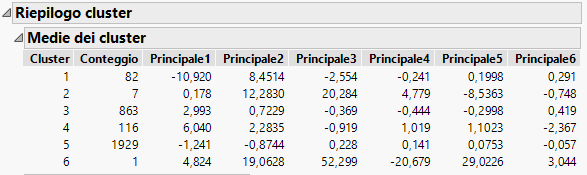
\includegraphics[width=0.30\textwidth]{Homework/Workload_Characterization/PCA_&_Clustering/6_Comp/Clustering/6_Cluster/Screen_Dati/Riepilogo.png}}
 	\subfigure{	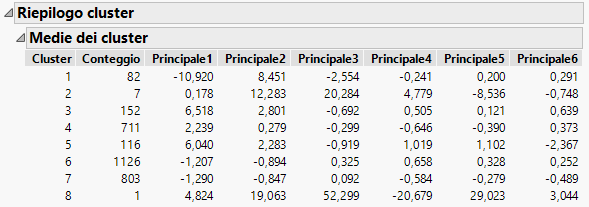
\includegraphics[width=0.30\textwidth]{Homework/Workload_Characterization/PCA_&_Clustering/6_Comp/Clustering/8_Cluster/Screen_Dati/Riepilogo.png}}
 	\subfigure{	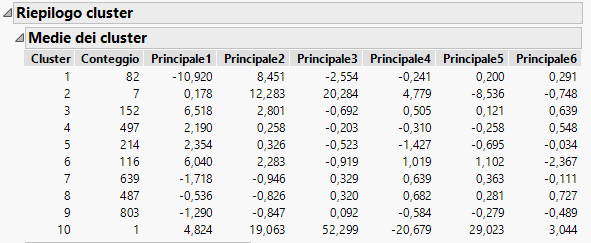
\includegraphics[width=0.30\textwidth]{Homework/Workload_Characterization/PCA_&_Clustering/6_Comp/Clustering/10_Cluster/Screen_Dati/Riepilogo.png}}
 	\subfigure{	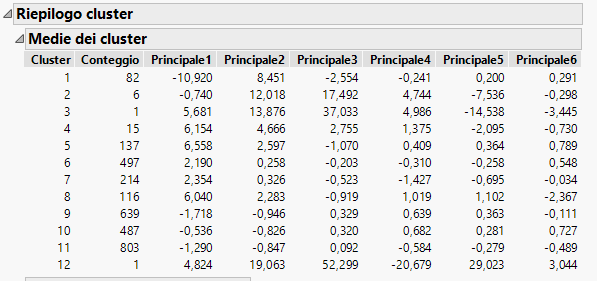
\includegraphics[width=0.30\textwidth]{Homework/Workload_Characterization/PCA_&_Clustering/6_Comp/Clustering/12_Cluster/Screen_Dati/Riepilogo.png}}
 	\subfigure{	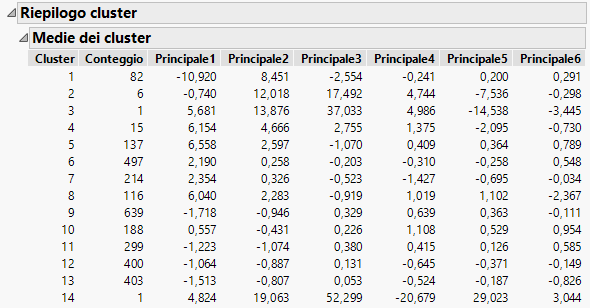
\includegraphics[width=0.30\textwidth]{Homework/Workload_Characterization/PCA_&_Clustering/6_Comp/Clustering/14_Cluster/Screen_Dati/Riepilogo.png}}
 	\subfigure{	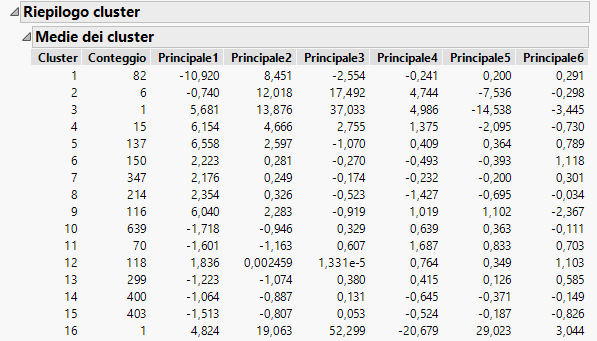
\includegraphics[width=0.30\textwidth]{Homework/Workload_Characterization/PCA_&_Clustering/6_Comp/Clustering/16_Cluster/Screen_Dati/Riepilogo.png}}
 	\caption{\textit{Numero di cluster e dimensione per diversi valori}}
 \end{figure}
 
 
 \begin{center}
 	\begin{tabular}{|c|c|c|c|c|c|}
 		\hline
 		\textbf{6 Cluster} & \textbf{8 Cluster} & \textbf{10 Cluster} &\textbf{12 Cluster}& \textbf{14 Cluster} & \textbf{16 Cluster} \\
 		\hline
 		22\% & 15\%& 13\% & 12\% & 11\% & 9\% \\
 		\hline
 	\end{tabular}
 \end{center}

\vspace{0.5cm}

\subsection{Interpretazione}
All'inizio dell'analisi sono state effettuate delle ipotesi che hanno trovato riscontro nella procedura di clustering:
\begin{enumerate}
	\item La fase iniziale del sistema (descritto dalle prime righe) trova riscontro con il cluster numero uno qualunque siano le componenti principali e qualunque sia il numero di cluster scelto. Questo quindi prova l'ipotesi definita inizialmente
	\item L'ultimo cluster contiene sempre un elemento singolo. Questo accade a causa del fatto che è stato identificato un picco nella fase iniziale delle misure. Esso inoltre è stato definito grazie all'outlier nel parametro Slab che non è stato eliminato, di conseguenza il picco viene racchiuso in un unico cluster in tutte le situazioni.
\end{enumerate}
\vspace{0.5cm}
In conclusione si può costruire una tabella che racchiude le informazioni riguardanti le PCA e la clusterizzazione in termini di percentuale di devianza persa.
 \begin{center}
	\begin{tabular}{|c|c|c|c|c|c|c|}
		\hline
		& \textbf{6 Cluster} & \textbf{8 Cluster} & \textbf{10 Cluster} &\textbf{12 Cluster}& \textbf{14 Cluster} & \textbf{16 Cluster} \\
		\hline
		\textbf{4 PC} & 26\%& 17\% & 16\% & 15\% & 14.5\% & 14\% \\

	\textbf{5 PC} & 25.5\%& 16\% & 15\% & 12\% & 11\% & 10\% \\

		\textbf{6 PC} & 22\% & 15\%& 13\% & 12\% & 11\% & 9\% \\
		\hline
	\end{tabular}
\end{center}

\newpage
\section{Workload Sintetico}
Come anticipato nel paragrafo precedente, sono state scelte 5 PC e per non perdere troppa varianza ma al tempo stesso non sfociare in un numero di cluster molto elevato, si è scelto di considerare 10 cluster. In tal caso la perdita di devianza con PCA e Cluster è di circa del 15\%.
\\In conclusione dopo aver calcolato i centroidi con uno script MATLAB il workload sintetico risulta essere:
\begin{figure}[H]
	\centering
	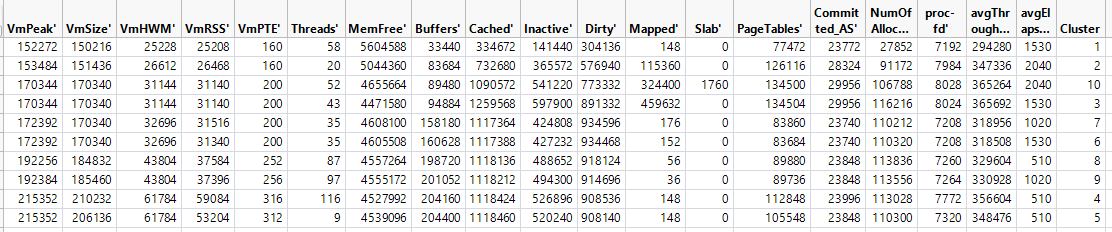
\includegraphics[width=\textwidth]{img/hw1/workload_sintetico.png}
	\caption{\textit{Workload sintetico}}
\end{figure}